\documentclass[red]{../tutorial}
\usepackage[no-math]{fontspec}
%\usepackage{xpatch}
%	\renewcommand{\ttdefault}{ul9}
%	\xpatchcmd{\ttfamily}{\selectfont}{\fontencoding{T1}\selectfont}{}{}
%	\DeclareTextCommand{\nobreakspace}{T1}{\leavevmode\nobreak\ }
\usepackage{polyglossia} % English please
	\setdefaultlanguage[variant=us]{english}
%\usepackage[charter,cal=cmcal]{mathdesign} %different font
%\usepackage{avant}
\usepackage{microtype} % Less badboxes


\usepackage[charter,cal=cmcal]{mathdesign} %different font
%\usepackage{euler}
 
\usepackage{tikz}
\usepackage{pgfplots}
\usetikzlibrary{arrows.meta}

\usepackage{blindtext}
\usepackage{calc, ifthen, xparse, xspace}
\usepackage{makeidx}
\usepackage[hidelinks, urlcolor=blue]{hyperref}   % Internal hyperlinks
\usepackage{mathtools} % replaces amsmath
\usepackage{bbm} %lower case blackboard font
\usepackage{amsthm, bm}
\usepackage{thmtools} % be able to repeat a theorem
\usepackage{thm-restate}
\usepackage{graphicx}
\usepackage{xcolor}
\usepackage{multicol}
\usepackage{fnpct} % fancy footnote spacing

 
\newcommand{\xh}{{{\mathbf e}_1}}
\newcommand{\yh}{{{\mathbf e}_2}}
\newcommand{\zh}{{{\mathbf e}_3}}
\newcommand{\R}{\mathbb{R}}
\newcommand{\Z}{\mathbb{Z}}
\newcommand{\N}{\mathbb{N}}
\newcommand{\proj}{\mathrm{proj}}
\newcommand{\Proj}{\mathrm{proj}}
\newcommand{\Perp}{\mathrm{perp}}
\newcommand{\Span}{\mathrm{span}\,}
\newcommand{\Img}{\mathrm{img}\,}
\newcommand{\Null}{\mathrm{null}\,}
\newcommand{\Range}{\mathrm{range}\,}
\newcommand{\rref}{\mathrm{rref}}
\newcommand{\Rank}{\mathrm{rank}}
\newcommand{\nnul}{\mathrm{nullity}}
\newcommand{\mat}[1]{\begin{bmatrix}#1\end{bmatrix}}
\renewcommand{\d}{\mathrm{d}}
\newcommand{\Id}{\operatorname{id}}



\theoremstyle{definition}
\newtheorem{example}{Example}[section]
\newtheorem{defn}{Definition}[section]

%\theoremstyle{theorem}
\newtheorem{thm}{Theorem}[section]

\pgfkeys{/tutorial,
	name={Tutorial 3},
	author={Bernardo Galv\~ao-Sousa},
	course={APM 348},
	date={},
	term={},
	title={Optimization}
	}

\begin{document}
	\begin{tutorial}
				\begin{objectives}
			In this tutorial you will explore some modelling towards optimization problems and using the techniques we have learned to analyze the results.

				These problems relate to the following course learning objectives:
				\begin{itemize}\it 
					\item Model with ODEs. \\[-20pt]
					\item Use Jupyter Notebook to approximate the solution. \\[-20pt]
					\item Create a visualization of the problem and the solution.
				\end{itemize}
%						\textit{Apply linear algebra techniques to classify solutions of linear systems of ordinary differential
%			equations including rigorously classifying the stability of equilibrium solutions and creating
%			linear approximations to non-linear systems of ordinary differential equations.}
		\end{objectives}

\vspace{-.5em}
\subsection*{Problems}
\vspace{-.5em}


\begin{enumerate}
	\item\label{q1} A bee goes from flower to flower to get pollen.
	
	At some point it has to decide when it advantageous to move to a different flower.
	
	Assume the following:
	\begin{itemize}
		\item Let $t$ be the time in minutes since the bee landed in the current flower.
		\item When the bee settles into a flower, it is full of pollen.
		\item The bee starts gathering its pollen at a rate proportional to the amount of pollen left in the flower (with proportionality constant 1).
		\item It takes 1 minute for the bee to find a new flower full of pollen.
	\end{itemize}
	
	\begin{enumerate}
		\item Find a function for the amount of pollen the bee has gathered since it landed on a flower.

		\textbf{Hint. } Keep track of the fraction of pollen still in the flower.
		


		\item Calculate the average rate of pollen gathering by the bee starting from the time the bee left the previous flower until time $t$.



		\item The bee decides to move on to the next flower when the average rate of pollen gathering starts decreasing. At what time does that happen?

		
%		\item Observe that at first the bee collects pollen rapidly, but it starts collecting pollen slower and slower.
%		
%		At some point, the rate at which the bee is collecting pollen becomes smaller than the average rate since it left the previous flower.
%		
%		That is the moment the bee decides to leave the flower to find another one still full of pollen.
%		
%		What is that time $t^\star$?
		

	\item Consider the following figure
	\begin{center}
		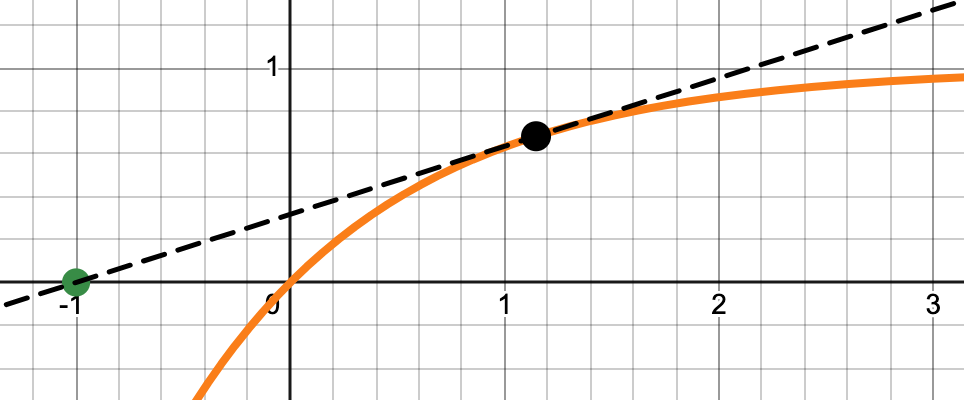
\includegraphics[width=.5\textwidth]{bees.png}
			% https://www.desmos.com/calculator/muodwklknf
	\end{center}
	
	Explain how it relates to this problem.

	\end{enumerate}
	
	

\newpage

\item \label{q2} Let us find a formula for the air density $\rho(y)$ at an altitude of $y$ metres.

\begin{enumerate}

	\item Consider the following two premises:
	\begin{itemize}
		\item[($P_1$)] Air density $\rho$ (in kg/m$^3$) is proportional to air pressure $p$ (in Pa), with proportionality constant $\frac{M}{RT}$, where:
		\begin{itemize}
			\item $M = $ molar mass of dry air $= 0.0289644$ kg/mol
			\item $R = $ ideal gas constant $= 8.31447$ J/(mol$\cdot$K)
			\item $T = $ temperature of the air (assuming it is constant)
		\end{itemize}
		\item[($P_2$)] Air pressure $p$ is the weight of the air above
	\end{itemize}
	
	For each premise, find a relation the air density with the air pressure.
	
	
	\item Using these two relations, obtain an equation for the air density $\rho(y)$. Then obtain a differential equation for the air density $\rho(y)$.
	
	
	\item Solve this differential equation to obtain a formula for the air density $\rho(y)$ assuming that $\rho(y_0) = \rho_0$.
	
	
	\item Use this formula to calculate the mass of Earth's atmosphere.
	
	\begin{minipage}{.7\textwidth}
	Here are some (simplified) facts that will help you:
	\begin{itemize}
		\item The \textbf{troposphere} and \textbf{stratosphere} contain 99.9\% of the mass of the atmosphere\\
	
%	Troposhpere facts:
		\item The temperature in the \textbf{troposphere} decreases linearly with altitude and
		\begin{itemize}
			\item $T_0=$ standard temperature at sea level $=288.15$ K
			\item $L=$ temperature lapse $ = 0.0065$ K/m
		\end{itemize}
		\item Air pressure in the \textbf{troposphere} is given by
			\[ p_T(h) = 	p_0 \left( 1 - \frac{Lh}{T_0} \right)^{\frac{gM}{RL}}\]
			where $h=$ altitude above sea level and $p_0=$ is the standard air pressure at sea level $= 101.325$ kPa \\
	
%	Stratosphere facts:
		\item The temperature in the \textbf{stratosphere} is constant.
	\end{itemize}
	\end{minipage}
	\hfill
	\begin{minipage}{.3\textwidth}
		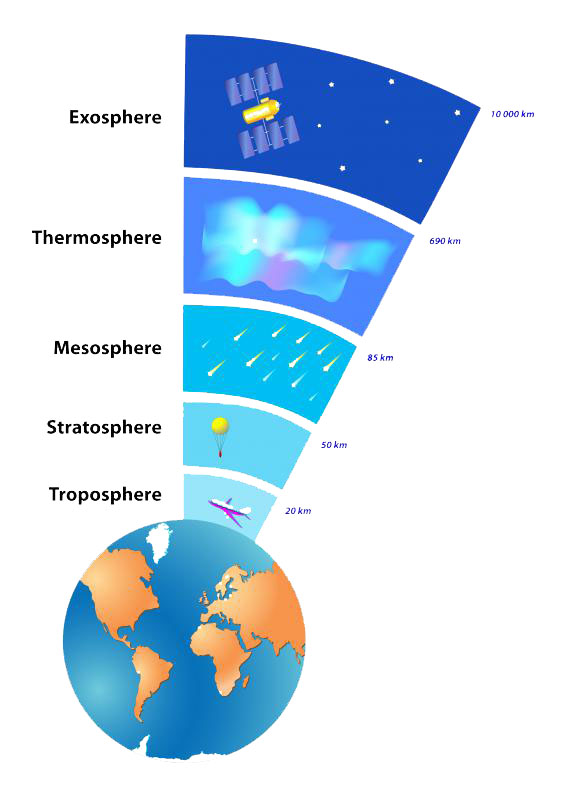
\includegraphics[width=\textwidth]{atmosphere.jpg}
	\end{minipage}

	\item It is often said that the Toposphere contains three quarters of the atmosphere's mass. Using the International Standard Atmosphere\footnote{\url{https://en.wikipedia.org/wiki/International_Standard_Atmosphere}}, check whether this model satisfies this.
	
	\item Compare this to the actual mass of the atmosphere. How can it be improved?

	
\end{enumerate}


	
	
	
	
\end{enumerate}


















	\end{tutorial}

	\begin{solutions}
		\begin{enumerate}

\item 
\begin{enumerate}
\item 
Let $p_f(t) = $ fraction of pollen in the flower at time $t$, so $p_f(0)=1$.

Let $p_b(t)=$ be the amount of pollen gathered by the bee from the current flower at time $t$. Thus $p_b(0)=0$.

We then have:
\[
\begin{cases}
	p_b' =  p_f \\	
	p_f' = - p_f
\end{cases}
\]

We can solve this system:
\[
\begin{cases}
	p_f(t) = e^{-t} \\
	p_b(t) = 1- e^{-t}
\end{cases}
\]


\item 
Average rate of pollen gathering $= \dfrac{\text{total amount of pollen}}{\text{time spent}} = \dfrac{p_b(t)}{1+t} = \dfrac{1-e^{-t}}{1+t}$.

\item The bee wants to maximize the average rate calculated before, so we want to solve the optimization problem:
\[
\max_{t \geq 0} \dfrac{1-e^{-t}}{1+t}
\]

So we need to find the solution of $f'(t)=0$:
\begin{align*}
f'(t) 	= \frac{e^{-t}(1+t) - (1-e^{-t})}{(1+t)^2} 
		  = \frac{(2+t)e^{-t} - 1}{(1+t)^2} & = 0 \\
\Leftrightarrow \quad (2+t)e^{-t} - 1 & = 0
\end{align*}

Solve using Newton's Method.
Get $t= 1.1461932206205825$.



\item 

\end{enumerate}



\newpage

\item 
\begin{enumerate}
\item From the first premise we have:
\[ \rho(y) = \frac{M}{RT} p(y) \]

From the second premise we get:
\[
	p(y) 	= \text{weight of the air above } y
			= g \int_y^\infty \rho(s) ~ds
\]


\item We get the equation
\begin{align*}
	\frac{RT}{M} \rho(y) & = g \int_y^\infty \rho(s) ~ds \\
	\frac{RT}{M} \frac{d\rho}{dy}(y) & = - g \rho(y) \\
	\frac{d\rho}{dy}(y) & = - \frac{gM}{RT} \rho(y)
\end{align*}
where we used the fact that $\displaystyle\lim_{y \to \infty} \rho(y) = 0$.


\item This is a first-order linear ODE, which is also a separable ODE, so we can solve it using either of the methods for these types of ODEs. 
We get:
\[ 
\rho(y) = \rho_0 e^{-\frac{gM}{RT} (y-y_0)}
\]
		

\item We have two regions to consider:

\paragraph{Troposphere.} In this region, we have
\begin{align*}
T(y) & = T_0 - y L \\
\rho_T(y) & = \frac{M}{R\cdot T(y-R_E)} p_T(y-R_E)
	= \frac{M}{R\cdot T(y-R_E)} p_0 \left( 1 - \frac{L(y-R_E)}{T_0} \right)^{\frac{gM}{RL}}
\end{align*}
where $R_E$ is the standard radius of the Earth $= 6\,378\,000$ m.

To calculate the mass of the troposphere, we need to integrate the air density the gravitational constant $g$ times the ``infinitesimal'' volume of each layer of atmosphere at altitude $y$: $4 \pi y^2 dy$. We get 
\[ 
M_T = \int_{R_E}^{R_T} 4 \pi y^2 g\rho_T(y) ~dy
\]
where $R_T = R_E + 20\,000$ m

\paragraph{Stratosphere.} The air density formula we calculated above, holds true in this region because the temperature is constant. The temperature here is
\[ 
T_S = T_0 - 20\,000 L = 158.15 {\rm K}.
\]
Which means that we have
\[
\rho_S(y) = \rho_T(20\,000) e^{-\frac{gM}{RT_S} (y-20\,000)}
\]

The mass of the stratosphere is
\[
M_S = \int_{R_T}^{R_S} 4 \pi y^2 g\rho_S(y) ~dy
\]
where $R_S = R_T + 30\,000 = R_E + 50\,000$ m.

We calculate this to get
\[
M = M_T + M_S \approx 5.19 \cdot 10^{19} \text{ kg}
\]


\item We can do the same calculations, using only the integral for $M_T$ up to $R_E+11\,000$ to  estimate the percentage of the atmosphere that is in the troposphere: We get 78\%, which is  pretty close to three quarters.

\item Another way to calculate the mass of the atmosphere\footnote{which is basically cheating because the standard sea level air pressure is defined to give the correct value for the mass of the atmosphere.}:

The air pressure at sea-level is 101325 Pa $=$ 101325 N / m$^2$, which means that the air above is exerting a weight of $ \frac{101325}{g}$ kg in each $m^2$ of Earth's surface.

That means that the total mass of the atmosphere is just multiplying this quantity by the surface area of the Earth:
\[
M = \frac{101325}{g} 4 \pi R_E^2 = 5.28 \cdot 10^{18} \text{ kg}.
\]

Our estimate is off by one order of magnitude.


\end{enumerate}


\newpage

%
%
%Temperature Lapse Rate
%
%\begin{tabular}{c|c|c}
%Altitude Region	& Lapse rate & $T(y)$\\
%(m)	& (K / km) & (K) \\ \hline
%0   -- 11\,000	  	& $6.5$ & $T(y)=288.15 -  0.0065 y$\\
%11\,000 -- 20\,000	& $0.0$ & $T(y) = 216.65$ \\
%20\,000 -- 32\,000	& $-1.0$ & $T(y) = 216.65 + 0.001 (y-20\,000)$ \\
%32\,000 -- 47\,000	& $-2.8$ & $T(y) = 228.65 + 0.0028 (y-32\,000)$\\
%47\,000 -- 51\,000	& $0.0$ & $T(y) = 270.65$ \\
%51\,000 -- 71\,000	& $2.8$	& $T(y) = 270.65 - 0.0028 (y-51\,000)$\\ 
%71\,000 -- 85\,000	& $2.0$ & $T(y) = 214.65 - 0.002 (y-71\,000)$
%\end{tabular}
%

\end{enumerate}
	

	
	\end{solutions}
	\begin{instructions}
		\subsection*{Learning Objectives}
	Students need to be able to\ldots
	\begin{itemize}
		\item Model with ODEs. \\[-20pt]
		\item Use Jupyter Notebook to approximate the solution. \\[-20pt]
		\item Create a visualization of the problem and the solution.
	\end{itemize}

\subsection*{Context}
	
In lecture we started studying some modelling with ODEs. 
In this tutorial, we will practice some more modelling and acting on the models to understand the phenomena better.


\paragraph{Important.} Don't rush problem 1 to be able to get to problem 2. 


\subsection*{Resources for TAs}

Some \texttt{Jupyter Notebook} scripts:
	\href{https://utoronto.syzygy.ca/jupyter/user-redirect/git-pull?repo=https://github.com/bigfatbernie/IBLMathModeling&subPath=tutorials/tutorial3/tutorial3.ipynb}{\tt tutorial3.ipynb}


\subsection*{Before Tutorial}

Send an announcement to students letting them know that they will need to bring a laptop and will be using Jupyter Notebooks \url{https://utoronto.syzygy.ca}.


\subsection*{What to Do}
	
Introduce the learning objectives for the day's tutorial.

Have students get into small groups and start on \#1 -- each group needs to have at least 1 laptop. \\

Problem \ref{q1}(c)-(d) are hard. Using the Desmos \url{https://www.desmos.com/calculator/xxswtammtc}, and letting $t$ increase, we can observe the dashed line that connects the amount of pollen the bee has connected to the moment the bee left the previous flower.
The average rate of pollen gathering is the slope of that line, so we can see that the line gets steeper and steeper until the moment when it becomes tangent to the orange ``pollen'' curve. At that point, it is more advantageous for the bee to stop collecting pollen and to move to the next flower.

\textit{Hint for students. } How can you visualize the average rate of pollen gathering in the drawing? 


	
\hfill 



In Exercise \label{q2}, here is some analysis of units for the ideal gas equation: $\rho = \dfrac{Mp}{RT}$:

\begin{itemize}
	\item $101.325$ J $  = 1$ atm L \quad and \quad $1$ atm $= 101325$ Pa
	\item $\left[\dfrac{Mp}{RT}\right] = \dfrac{kg}{J \cdot Pa} = \dfrac{kg}{1000 L} = \dfrac{kg}{m^3} = [\rho]$
\end{itemize}



%
%	
%	rho = Mp/RT  with  p in Pa
%	
%	
%	p = atm = 101.325 kPa
%	
%	101.325 J = 1 atm L
%		
%	Mp / RT = kg / J  * Pa
%			= 101.325 kg / ( atm L ) * atm / 101325
%			= kg / (1000L)
%	rho	= kg / m^3
%			
%	




%\subsection*{Notes}
%
%	\begin{enumerate}
%		\item Note
%	\end{enumerate}
	
	

	
	

	\end{instructions}

\end{document}
